\documentclass{article}
\usepackage{graphicx, soul, amsmath}
\usepackage[dvipsnames]{xcolor}
\usepackage[a4paper, margin=0.8in]{geometry}
\usepackage{fancyhdr} % Paquete para encabezados y pies de página

% Configuración de soul
\setul{0.5ex}{0.3ex}

% Comandos personalizados
\newcommand{\ulcolor}[2][Red]{\setulcolor{#1}\ul{#2}}
\newcommand*\sepline{%
  \begin{center}
    \rule[1ex]{.5\textwidth}{.5pt}
  \end{center}}

% Configuración de encabezado y pie de página para todas las páginas
\fancypagestyle{main}{
    \fancyhf{} % Limpia encabezados y pies de página
    \fancyhead[C]{Juan Ignacio Elosegui} % Encabezado centrado con tu nombre
    \fancyfoot[R]{\thepage} % Número de página alineado a la derecha en el pie
    \renewcommand{\headrulewidth}{0.4pt} % Línea bajo el encabezado
    \renewcommand{\footrulewidth}{0pt}   % Sin línea en el pie de página
}

% Aplicar el estilo por defecto a todo el documento
\pagestyle{main}

\title{Teoría de las Decisiones $-$ Comportamiento (Resumen)}
\date{Noviembre 2024}

\begin{document}

    % Primera página con título y encabezado
    \maketitle
    \thispagestyle{main} % Asegura el estilo en la primera página
    
\section*{\underline{Módulo I: Teoría de Juegos}}
    \subsection*{\textbf{Clase I: Dixit Cap. 2 página 18 a 36}}
        No incluí todo lo que es de características de los juegos y los tipos de juegos. Con saberlos alcanza.
        \\
        Cuando una persona decide cómo actuar cuando trata con otra gente (o equipos o firmas), debe haber algún efecto de sus acciones; lo que uno hace, debe afectar a la decisión de algún otro.

        Para que la interacción se convierta en un juego estratégico, necesitamos que los participantes \emph{sean conscientes de este efecto colateral}.

        Esta distinción en las interacciones las convierte en \emph{juegos estratégicos} entre jugadores cuyas decisiones serán tomadas sin importar la reacción o la respuesta de los otros.

    
    \subsection*{\textbf{Clase II: Dixit Cap. 4, página 91 a 98}}
        Se dice que los juegos son simultáneos si los jugadores deciden sin conocer las decisiones de los otros jugadores, si los jugadores deciden sus acciones al mismo tiempo, y también si deciden de manera aislada (sin saber lo que los otros jugadores hicieron o sin saber lo que van a hacer).
        \\
        \\
        En muchos juegos, cada jugador tiene disponible un número de \emph{estrategias puras} posibles -como puede ser llevar la pelota, hacer un pase o patear al arco en fútbol-. En otros juegos, las estrategias puras de cada jugador puede ser un número de un rango continuo (como puede ser un precio que pone una firma). Esta distinción no hace ninguna diferencia al concepto de \emph{equilibrio} en los juegos simultáneos, pero suele ser más fácil encontrarlo con estrategias puras que con estrategias continuas.

        Los juegos simultáneos con estrategias puras se pueden ver en matrices de juego o cuadro de pagos. Este cuadro es la \emph{forma normal} del juego.

        \begin{center}
            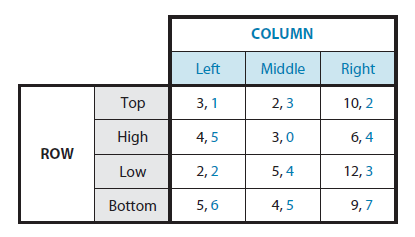
\includegraphics[width=0.5\linewidth]{figs/fig9.PNG}
        \end{center}

        Los jugadores se llaman Row y Column. Row tiene 4 estrategias posibles: Top, High, Low y Bottom; mientras que Column tiene 3 estrategias posibles: Left, Middle y Right. Cada selección de Row y Column genera un resultado potencial del juego. Los pagos asociados con cada resultado están en la celda correspondiente a esa fila y esa columna.
        \\
        \\
        A veces, los pagos podrían sumar cero. Este patrón es muy común en los deportes, donde los intereses de los dos lados son exactamente opuestos uno de otro. A estos juegos se les dice \emph{juegos de suma cero}.
        \\
        \\
        Para analizar los juegos simultáneos, hay que considerar cómo los jugadores eligen sus acciones. En la Figura 1, cuando Row elige Low y Column elige Middle, el pago es de 5 para Row y 4 para Column.

        Como Row eligió Low, ¿puede Column hacer algo mejor en vez de elegir Middle? No, porque Left le daría un pago de 2, y Right le daría un pago de 3, de los cuales ninguna de esas opciones le paga mejor que Middle. Así, Middle es la \emph{mejor respuesta} para Column cuando Row elige Low. De manera análoga, Low is la \emph{mejor respuesta} de Row si Column elige Middle, porque ninguna otra opción paga mejor.

        Estas dos opciones tienen la propiedad de que son la mejor respuesta en función de la decisión del otro. Si hicieran los dos esas opciones (Middle, Low) no eligirían otra cosa. Como en esa situación, nadie tiene incentivos para elegir otra estrategia, se le llama \emph{Equilibrio de Nash}. Un equilibrio de Nash es un conjunto de estrategias para cada jugador, en el cual ningún jugador puede recibir un pago mayor si elige otra estrategia.
    
    \subsection*{\textbf{Clase III: Dixit Cap. 4, página 99 a 112}}
        Algunos juegos tienen la propiedad de que una estrategia es uniformemente mejor o peor que otra. Cuando pasa esto, provee una manera en la cual la búsqueda del Equilibrio de Nash se puede simplificar.

        El \emph{Dilema del Prisionero} ilustra bien esto.

        \begin{center}
            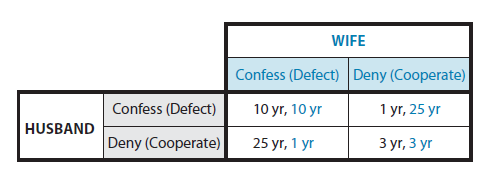
\includegraphics[width=0.5\linewidth]{figs/fig10.PNG}
        \end{center}
        
        El Marido y la Esposa están en un juego simultáneo (Dilema del Prisionero) en el cual tienen que elegir entre confesar o no confesar un asesinato. Los dos saben que no confesar implica que reciben una condena de 3 años por el secuestro. También saben que, si uno de ellos confesa, sólo el que confesó recibe 1 año de condena por colaborar con la policía, mientras el otro recibirá una condena de 25 años mínimo.

        Acá, entre menor sea el pago, mejor, así que los dos preferirían opciones como esas.
        \\
        \\
        El Marido tiene que pensar \emph{lo que la Esposa va a hacer}. Suponé que el Marido cree que su Esposa va a confesar, entonces su mejor opción es confesar - recibe 10 años de condena, en vez de 25 si es que no hubiera confesado. Si cree que la Esposa no va a confesar, su mejor opción es confesar, ya que recibe 1 año en vez de recibir 3 si él no hubiese confesado.

        En este juego, confesar es mejor que no confesar para el Marido \emph{sin importar lo que piense que eligió su Esposa}. Esto significa que -para el Marido- la estrategia Confesar es una \emph{estrategia dominante} o que la estrategia No Confesar es una \emph{estrategia dominada}. Podemos decir también que la estrategia Confesar \emph{domina} a la estrategia No Confesar o que No Confesar \emph{está dominada} por Confesar.

        Si un jugador actúa racionalmente (como es de asumir) no hay razón para que el jugador elija una estrategia que sea mala, sin importar lo que el otro puede estar eligiendo. Y, si el jugador sabe que una estrategia es claramente mejor, siempre la elegirá. Gallardo va a poner a Kranevitter en cancha, porque claramente es mejor que Villagra (por ejemplo). Pero todo es parte de la estrategia, ¿no?

        La dominancia debería hacer que el Marido confiese. Lo mismo aplica para su Esposa: Confesar domina a su potencial estrategia No Confesar; entonces también suponemos que elija Confesar. Así, (Confesar, Confesar) es el resultado predicho para este juego. Este es el Equilibrio de Nash -el único en el juego-.
        \\
        \\
        Los juegos que vimos hasta ahora tenían dos estrategias puras para cada jugador nada más. En estos juegos, si una estrategia es dominante, la otra será la dominada; entonces elegir la dominante es lo mismo que ni siquiera considerar la dominada -es decir, \emph{eliminarla}-. Si los jugadores se encuentran en juegos como estos, pueden encontrar el equilibrio eliminando las estrategias dominadas de la consideración.
        
        La \emph{eliminación sucesiva} or \emph{eliminación iterada de estrategias dominadas} usa este proceso de remoción de estrategias dominadas y reduce el tamaño del juego a su mínima expresión. Si este proceso resulta en una única estrategia, el juego se puede \emph{resolver por dominancia}, y esa estrategia será el Equilibrio de Nash.
        \\
        \\
        Muchos juegos simultáneos no tienen estrategias dominantes, y, por lo tanto, no tendrán estrategias dominadas tampoco. Otros pueden tener una o más estrategias dominadas, pero la eliminación sucesiva de estrategias no nos puede llevar siempre a una única solución. Para encontrar la solución de juegos como estos, asumimos que las creencias de los jugadores son correctas. Luego, vemos la perspectiva de cada jugador en su turno y preguntarnos lo siguiente: para cada una de las opciones que los otros jugadores podrían estar haciendo, ¿cuál es la mejor opción para este jugador? Así, encontramos las \emph{mejores respuestas} para cada jugador, considerando todas las estrategias posibles de los demás.

        La \emph{mejor respuesta} de un jugador es la estrategia (o conjunto de estrategias) que le paga lo máximo posible al jugador, dadas las estrategias de los demás.
        \\
        \\
        Vimos juegos que tienen un Equilibrio de Nash con una única estrategia pura, pero no pasa siempre esto - pueden haber múltiples Equilibrios de Nash. Estos juegos son los \emph{juegos de coordinación}, porque los jugadores tienen intereses en común, como puede ser que dos personas se encuentren en un bar en una hora estipulada.

\section*{\underline{Módulo II: Estrategias Mixtas}}
    \subsection*{\textbf{Clase V: Dixit Cap. 7, página 185 a 216}}
        Los jugadores pueden decidir actuar de manera aleatoria a la hora de elegir sus estrategias puras, para que no sean tan predecibles y que el otro sepa siempre cómo actuar en manera de respuesta.
        
        \begin{center}
            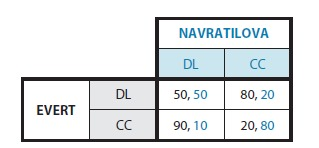
\includegraphics[width=0.5\linewidth]{figs/fig11.jpeg}
        \end{center}
        
        En la imagen tenemos un partido de tenis (un juego de suma cero) en el cual los dos jugadores tienen intereses opuestos. Evert quiere pegarle derecho (DL) o cruzado (CC), al lugar donde no esté Navratilova. Navratilova quiere estar en la dirección en la que Evert le pegue a la pelota. Cualquier decisión sistemática (es decir, que haga siempre lo mismo) de Evert será aprovechada por Navratilova para su ventaja, lo que termina siendo una desventaja para Evert. Por eso, Evert puede actuar de manera \emph{aleatoria}.

        Como toman sus decisiones de manera no-sistemática (aleatoria), eligen entre sus estrategias puras. Navratilova y Evert eligen entre pegarle derecho (DL) o cruzado (CC). Llamamos a la "mezcla" aleatoria entre esas dos estrategias puras una \emph{estrategia mixta}.

        Antes, habíamos visto que los jugadores eligen una estrategia pura con una probabilidad discreta de $[0, 1]$. Es decir, o la eligen o no.

        Permitir estrategias mixtas en un juego resuelve el problema de la posible no existencia del Equilibrio de Nash, por lo que en juegos con mixtas siempre habrá algún equilibrio.
        \\
        \\
        Para hallar el Equilibrio de Nash, tenemos que analizar la mejor respuesta. Primero, tenemos que identificar la mejor respuesta de Evert para cada estrategia mixta posible de Navratilova.
    
        \newpage
        
        \begin{enumerate}
            \item Encontramos el pago esperado de Evert:
                \begin{center}
                    $50p+90(1-p)$ si Navratilova elige jugar derecho (DL), y
                    \\
                    $80p+20(1-p)$ si decide jugar cruzado (CC).
                \end{center}
            \item Contra el $q$-mix de Navratilova, el pago esperado de Evert es:
                \begin{center}
                    $[50p+90(1-p)] \cdot q + [80p+20(1-p)] \cdot (1-q) = $
                    \\
                    $[20+70q] + [60-100q] \cdot p$
                \end{center}
            \item Usamos el pago esperado para que nos ayude a encontrar los valores de $p$ de la mejor respuesta de Evert. Tratamos de encontrar el $p$ que maximice el pago de Evert para cada valor $q$ de Navratilova, entonces conviene ver cómo varía el pago esperado de Evert si modificamos $p$. Lo que importa es el coeficiente en $p: [60-100q]$. Es más, importa si el coeficiente $60-100q$ es positivo o negativo, por lo que su signo depende de $q$. Por lo tanto, hallamos el valor crítico de $q$ que cumpla que:
                \begin{center}
                    $60-100q = 0$
                    \\
                    $q = 0.6$
                \end{center}
            \item Para Navratilova, si elige un $q < 0.6$, $[60-100q]$ es positivo, el pago esperado de Evert incrementa cuando $p$ incrementa, y la mejor decisión para Evert será $p = 1$, o sea, puramente jugar derecho (DL). Si Navratilova elige un $q > 0.6$, la mejor opción para Evert es que $p = 0$, o jugar cruzado (CC). Si Navratilova establece que $q=0.6$, Evert tiene el mismo pago esperado, sin importar el valor de $p$, y cualquier "mezcla" entre DL y CC será la mejor opción. Para resumir:
                \begin{center}
                    $q < 0.6 \Rightarrow p = 1$ (puramente jugar DL -derecho-)
                    \\
                    $q = 0.6 \Rightarrow$ cualquier $p$-mix es la mejor respuesta.
                    \\
                    $q > 0.6 \Rightarrow p = 0$ (jugar puramente CC -cruzado-)
                    \\
                \end{center}
            \begin{center}
                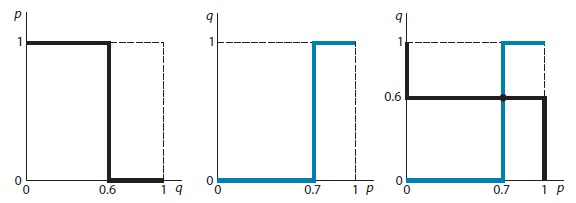
\includegraphics[width=0.5\linewidth]{figs/fig12.jpeg}                
            \end{center}
            \item Podemos ver que la mejor respuesta de Navratilova está en la imagen de arriba (sin hacer cálculos). Podemos ver que:
                \begin{center}
                    $p < 0.7 \Rightarrow q = 0$ (puro CC -cruzado-)
                    \\
                    $p = 0.7 \Rightarrow$ cualquier $q$-mix es la mejor respuesta.
                    \\
                    $p > 0.7 \Rightarrow q = 1$ (puro DL -derecho-)
                \end{center}
        \end{enumerate}
    
\section*{\underline{Módulo III: Juegos Secuenciales/Dinámicos}}
    Nota: la bibliografía cubre las clases 7, 8 y 9. No voy a dividir las clases, directamente voy a resumir la bibliografía.
    \subsection*{\textbf{Dixit Cap. 3}}
        En los juegos secuenciales hay situaciones estratégicas en las que hay un orden de juego establecido. En estos juegos los jugadores los jugadores tienen \emph{turnos} y saben qué hicieron los jugadores cuando les tocó jugar. Un juego secuencial puede ser el tateti o el ajedrez. Como es de esperar, los jugadores deben pensar cómo va a reaccionar su oponente respecto a la jugada que hicieron; es decir, deciden sus movimientos en base a cálculos de futuras consecuencias para los demás y para ellos mismos.
        \\
        \\
        En los juegos secuenciales usamos un \emph{árbol} para ver al juego de \emph{forma extensiva}. Estos árboles muestran todos los puntos de decisión (turnos), llamados nodos; y de ellos salen las ramas, que son las decisiones posibles en base a lo que sucedió en ese turno.
            \begin{itemize}
                \item En el juego de abajo, sabemos que Jugador 1 tiene el primer turno; por eso, está más a la izquierda, y se le dice \emph{nodo inicial} o \emph{raíz}. Como tiene dos decisiones posibles el Jugador 1 (jugar la Estrategia A o jugar la Estrategia B), también se cuenta como un nodo de decisión. Todas las ramas van a salir del nodo raíz.
                \begin{center}
                    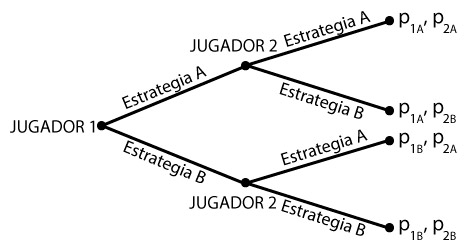
\includegraphics[width=0.5\linewidth]{figs/fig13.jpg}
                \end{center}
                \item Se puede trazar un número de distintos "caminos" posibles a través del árbol siguiendo las ramas.
                \item Como consideramos que estos juegos secuenciales sí tienen un fin, podemos ver que, al final de cada camino, llegamos al \emph{nodo terminal}, donde los jugadores no tienen más turnos.
                \item Cada línea que une los nodos se llama \emph{acción}. Los jugadores pueden planear las acciones que van a hacer entre todas las posibles eventualidades que sucedan (es decir, pensar para adelante según lo que haga el oponente). Este plan de acciones se llama \emph{estrategia}. Cabe aclarar que pueden existir errores a la hora de que un jugador haga una acción en su turno, como puede ser equivocarse.
            \end{itemize}
        Para poder encontrar el o los equilibrios del juego mirando un árbol voy a plantear un ejemplo en el cual probablemente muchos hayamos estado, \emph{si fumar o no}. Carmen tiene 16 años, no escuchó el consejo de sus padres, y está considerando fumar. Si prueba el cigarrillo, tiene el poder de decidir si sigue fumando o no.

        Consideremos los pagos: supongamos el escenario en el que ni siquiera prueba el cigarrillo, el cual tiene un pago de $0$. Como a Carmen le gusta experimentar con boludeces como estas de joven, por lo que habrá un escenario en el que sí probó el cigarrillo pero no sigue fumando que le ofrece un pago de $+1$. Pero, más allá de los problemas de salud que fuera a tener a largo plazo, su pelo y su ropa van a tener un olor horrible si es que prueba el cigarrillo y sigue fumando, lo que le representa un pago de $-1$.

        \begin{center}
            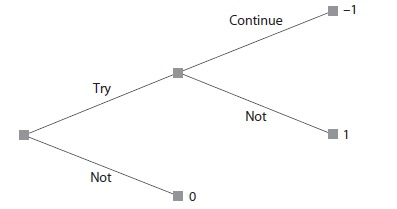
\includegraphics[width=0.5\linewidth]{figs/fig14.jpeg}
        \end{center}

        La mejor decisión de Carmen es clara: le conviene probar el cigarrillo, pero no seguir fumando.

        Puede parecer una estupidez, pero no estamos considerando el problema de la adicción. Si Carmen hubiera probado el cigarrillo por un largo tiempo, le puede ir agarrando el gusto y, por lo tanto, representando pagos distintos. Se podría decir que ahora en el juego existen dos (pseudo)jugadores: la Carmen del Hoy, y la Carmen del Mañana. La Carmen del Mañana decidirá si seguir fumando o no, luego de que la Carmen del Hoy haya decidido probar el cigarrillo o no. En la imagen de abajo se puede ver el nuevo formato del árbol: la Carmen del Hoy sana tiene marcados sus pagos con color azul y la Carmen del Mañana tiene sus pagos -casualmente- en negro.

        \begin{center}
            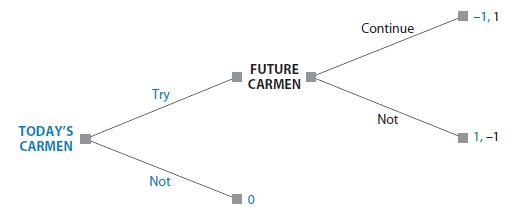
\includegraphics[width=0.5\linewidth]{figs/fig15.jpeg}
        \end{center}

        La Carmen del Mañana va a preferir continuar fumando. La Carmen del Hoy debería adelantarse a lo que va a hacer Carmen del Mañana, reconociendo que, si prueba el cigarrillo, le va a terminar haciendo mal si es que la Carmen del Mañana se hace adicta.

        No importa cómo visualices tu estrategia en el árbol, la lógica del análisis es el mismo y es importante. Tenés que empezar tu análisis considerando los nodos de acción que llevan directamente a los nodos terminales. La decisión óptima para un jugador en cualquier nodo puede ser encontrada de inmediato comparando sus pagos en los nodos terminales relevantes. A este método de pensar para adelante y razonar para atrás e llama inducción hacia atrás. La inducción hacia atrás nos ayuda a conseguir los Equilibrios Perfectos en Subjuegos.

    \subsection*{\textbf{Dixit Cap. 6}}
        Los juegos más comunes de juegos secuenciales y simultáneos a la vez son aquellos entre dos o más jugadores a lo largo de un período de tiempo. Los juegos como estos tienen la propiedad de que la acción de una persona está influenciada por el historial de tus acciones hasta ese momento y también influenciada por las expectativas de las interacciones por venir.

        Un \emph{subjuego} es un subconjunto de un árbol que contiene a todos sus nodos sucesores. Un jugador debe elegir su acción óptima en cada escenario que podría enfrentar (cada subjuego posible), ya que esperamos que ese escenario ocurra o no. Esto nos puede ayudar a encontrar los Equilibrios de Nash en juegos secuenciales con información perfecta o imperfecta.
        
\end{document}
